\documentclass[exercice]{thedocument}%
\usepackage{texmaths-tikz}%
\startdatakeys
\source{}
\cycle{}
\competencesDuSocle{}
\connaissancesRequises{}
\competencesTravaillees{}
\enddatakeys
\begin{document}%
Décrire en une phrase les figures suivantes :\vskip15pt
\begin{tikzpicture}[rotate=70]
    \coordinate[label=A](A)at(20:1.5);
    \coordinate[label=above right:B](B)at(-20:1.5);
    \coordinate[label=below:C](C)at(-160:1.5);
    \coordinate[label=left:D](D)at(160:1.5);
    \draw(A)--(B)--(C)--(D)--cycle;
    \tkzMarkRightAngle(A,B,C)
    \tkzMarkRightAngle(B,C,D)
    \tkzMarkRightAngle(C,D,A)
    \tkzMarkRightAngle(D,A,B)
\end{tikzpicture}\hskip10pt
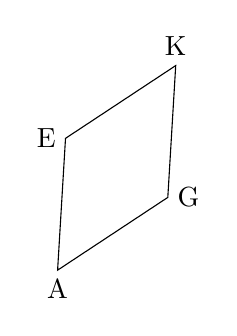
\begin{tikzpicture}[scale=0.75,rotate=-30]
    \coordinate[label=right:G](A)at(0:1);
    \coordinate[label=above:K](B)at(90:2);
    \coordinate[label=left:E](C)at(180:1);
    \coordinate[label=below:A](D)at(-90:2);
    \draw(A)--(B)--(C)--(D)--cycle;
    \tkzMarkSegment[mark=s||](A,B)
    \tkzMarkSegment[mark=s||](C,B)
    \tkzMarkSegment[mark=s||](C,D)
    \tkzMarkSegment[mark=s||](A,D)
\end{tikzpicture}\hskip10pt
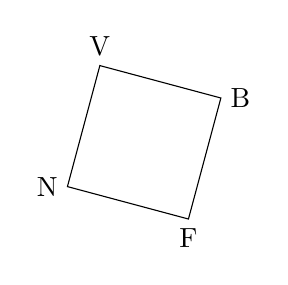
\begin{tikzpicture}[scale=0.75,rotate=30]
    \coordinate[label=right:B](A)at(0:1.5);
    \coordinate[label=above:V](B)at(90:1.5);
    \coordinate[label=left:N](C)at(180:1.5);
    \coordinate[label=below:F](D)at(-90:1.5);
    \draw(A)--(B)--(C)--(D)--cycle;
    \tkzMarkSegment[mark=s||](A,B)
    \tkzMarkSegment[mark=s||](C,B)
    \tkzMarkSegment[mark=s||](C,D)
    \tkzMarkSegment[mark=s||](A,D)
    \tkzMarkRightAngle(A,B,C)
    \tkzMarkRightAngle(B,C,D)
    \tkzMarkRightAngle(C,D,A)
    \tkzMarkRightAngle(D,A,B)
\end{tikzpicture}
\end{document}
